\documentclass[a4paper,10pt]{article}
%\documentclass[a4paper,10pt]{scrartcl}

\usepackage[pdftex=true,colorlinks=,plainpages=false]{hyperref} % Soporte hipertexto

\usepackage[utf8x]{inputenc}
\usepackage{graphicx}

\title{Modelo de diseño}
\author{Sigifredo Escobar Gómez}
\date{}

\pdfinfo{%
  /Title    (Modelo de diseño)
  /Author   ()
  /Creator  ()
  /Producer ()
  /Subject  ()
  /Keywords ()
}

\begin{document}
\maketitle Modelo de diseño

\tableofcontents	% Tabla de contenido
% \listoffigures		% Índice de figuras
% \listiftables		% Índice de tablas

\newpage

\section{sec1}


\section{sec2}


\section{sec3}

\section{Gestión}
\subsection{Lecciones aprendidas del diseño}
\subsection{Indicadores de gestión}
\subsubsection{Desviación de lo planeado vs lo ejecutado}

\begin{figure}[h!]
  \centering
    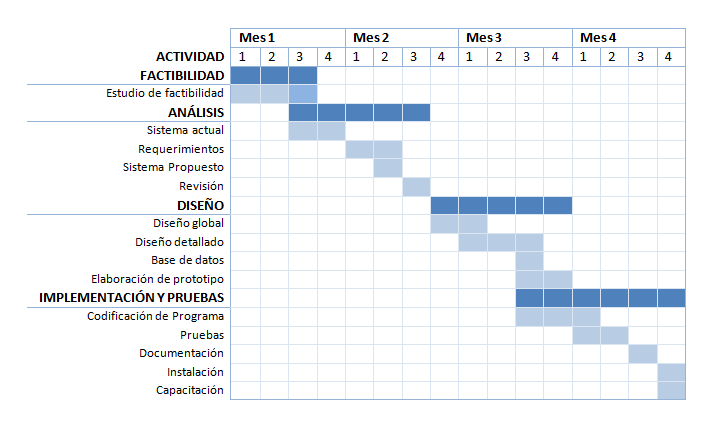
\includegraphics[width=0.80\textwidth]{./img/cal1.png}
  \caption{Plan de trabajo propuesto}
\end{figure}
 
\begin{figure}[h!]
  \centering
      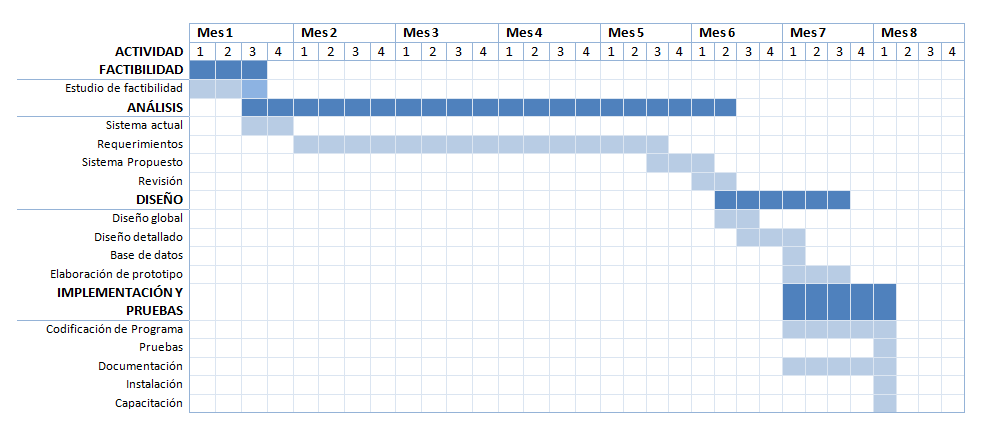
\includegraphics[width=0.80\textwidth]{./img/cal2.png}
  \caption{Plan de trabajo ejecutado}
\end{figure}

\maketitle En las figuras 1 y 2 podemos observar el plan propuesto al inicio del proyecto con el ejecutado. El desvío se devió a la situación que en ese momento ocurrida en la Universdad de Antioquia. Por esta razón el cliente pidió parar el desarrollo normal del proyecto hasta que se normalizara la situación y los estudiantes, profesores y grupos de investigación regresaran a su normal funcionamiento.

\subsubsection{Gráfica de valor ganado de proyecto}

\begin{center}
\begin{tabular}{| c | c | c | c |}
\hline
Tarea & Recurso humano & Recurso técnico & Total \\
\hline

\hline
\end{tabular}
\end{center}

\section{Soporte}
\subsection{Indicadores de soporte}
\subsection{Número de defectos de diseño hallados en verificación y validación}

\begin{figure}[h!]
  \centering
    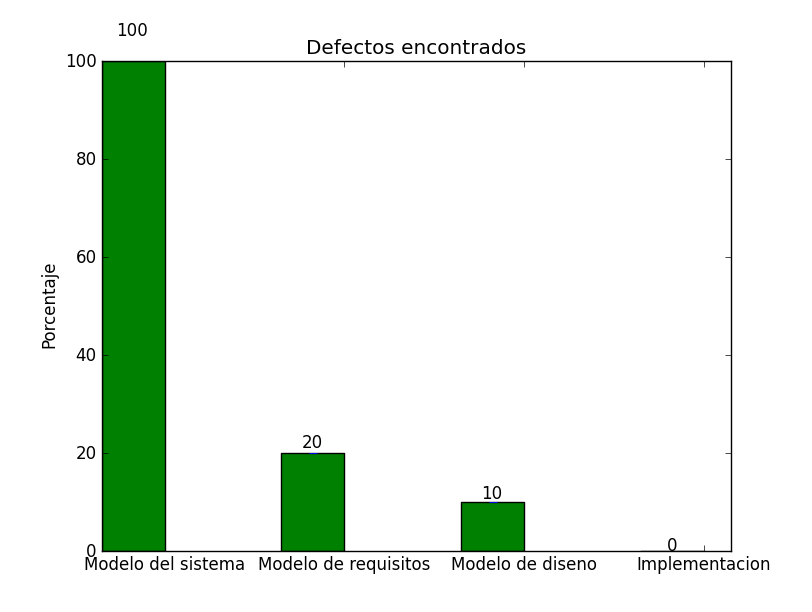
\includegraphics[width=0.80\textwidth]{./img/barras/barras.png}
  \caption{Defectos encontrados}
\end{figure}

\end{document}
